\documentclass[aspectratio=169,11pt,t]{beamer}
\usepackage[spanish]{babel}
\usepackage{graphicx}
\usepackage{booktabs}
\usepackage{xcolor}
\usepackage[backend=biber,style=ieee]{biblatex}
\graphicspath{{figuras/}}
\addbibresource{referencias.bib}

% Identidad visual del equipo: azul suave, fondo claro y espacio para diagramas.
\definecolor{azulProfundo}{HTML}{29475B}
\definecolor{azulMedio}{HTML}{5D8EAE}
\definecolor{azulClaro}{HTML}{EAF3F8}
\definecolor{azulLinea}{HTML}{B7CEDD}
\definecolor{textoSuave}{HTML}{516775}
\definecolor{fondo}{HTML}{FBFDFE}

\setbeamercolor{normal text}{fg=azulProfundo,bg=fondo}
\setbeamercolor{structure}{fg=azulMedio}
\setbeamercolor{frametitle}{fg=azulProfundo,bg=fondo}
\setbeamercolor{title}{fg=azulProfundo}
\setbeamercolor{subtitle}{fg=textoSuave}
\setbeamercolor{block title}{fg=azulProfundo,bg=azulClaro}
\setbeamercolor{block body}{fg=azulProfundo,bg=azulClaro}
\setbeamercolor{alerted text}{fg=azulMedio}
\setbeamercolor{bibliography entry author}{fg=azulProfundo}
\setbeamercolor{bibliography entry title}{fg=azulProfundo}
\setbeamercolor{bibliography entry location}{fg=textoSuave}
\setbeamercolor{bibliography entry note}{fg=textoSuave}

\setbeamerfont{frametitle}{size=\Large,series=\bfseries}
\setbeamerfont{normal text}{size=\normalsize}
\setbeamerfont{footline}{size=\scriptsize}
\setbeamerfont{block title}{series=\bfseries}
\setbeamersize{text margin left=1.05cm,text margin right=1.05cm}
\setlength{\parskip}{0.35em}

\setbeamertemplate{navigation symbols}{}
\setbeamertemplate{itemize item}{\color{azulMedio}\raisebox{0.15ex}{\scriptsize$\bullet$}}
\setbeamertemplate{itemize subitem}{\color{azulMedio}\scriptsize$\bullet$}
\setbeamertemplate{frametitle}{%
  \vspace*{0.33cm}%
  \insertframetitle\par
  \vspace{0.10cm}%
  {\color{azulLinea}\rule{\textwidth}{0.7pt}}%
}
\setbeamertemplate{footline}{%
  \hbox to \paperwidth{%
    \hspace{1.05cm}{\color{textoSuave}\usebeamerfont{footline}Aplicaciones Distribuidas}%
    \hfill
    {\color{azulMedio}\usebeamerfont{footline}\insertframenumber}%
    \hspace{1.05cm}%
  }%
  \vspace{0.25cm}%
}

% Para citar junto al dato o diagrama, por ejemplo: \fuente{clave_bib}.
\newcommand{\fuente}[1]{{\footnotesize\color{textoSuave}Fuente: \cite{#1}}}

\title{Computación paralela en un sistema distribuido real}
\subtitle{Sistema analizado: Apache Spark · aplicación al PFC: RTV}
\author{GARCIA SANGOQUIZA \and GIRALDO CAGUA \and HERRERA BARCO \and LOMBEIDA ESCALERAS}
\date{}
\begin{document}
% La identificación del equipo y del sistema debe integrarse en la diapositiva 1.
% No se agrega portada separada: hay 12 minutos para 12 diapositivas de contenido.
\begin{frame}{RTV: varias revisiones, un estado común}
  \vspace{-0.15cm}
  {\footnotesize García Sangoquiza \textbullet{} Giraldo Cagua \textbullet{}
  Herrera Barco \textbullet{} Lombeida Escaleras\par}
  \vspace{0.12cm}
  \begin{columns}[T,onlytextwidth]
    \begin{column}{0.61\textwidth}
      \begin{block}{Centro de revisión de Valencia}
        \small Gestiona turnos, pruebas y certificados.\\[0.12cm]
        Recepción, recaudación, inspectores y jefatura.
      \end{block}
    \end{column}
    \begin{column}{0.35\textwidth}
      \begin{block}{Alcance documentado}
        {\Large\bfseries 1 centro municipal}\\[0.10cm]
        \small Varias líneas: requisito RNF-08.\\
        {\scriptsize No hay carga real medida.}
      \end{block}
    \end{column}
  \end{columns}
  \vspace{0.08cm}
  {\small
  \textbf{Paralelismo:} ejecutar tareas al mismo tiempo.\\[0.10cm]
  \textbf{Distribución:} componentes que cooperan por red.\\[0.10cm]
  \textbf{En RTV:} concurrencia entre revisiones; CPU no verificada.\par}
  \vfill
  {\scriptsize Caso académico: backend y BD en nodos separados, por supuesto explícito.\par
  Fuentes: \cite{gs_rtv,gs_oracle_hilos}.}
\end{frame}

\begin{frame}{Arquitectura: quién coordina y dónde está el estado}
  \vspace{-0.12cm}
  \centering
  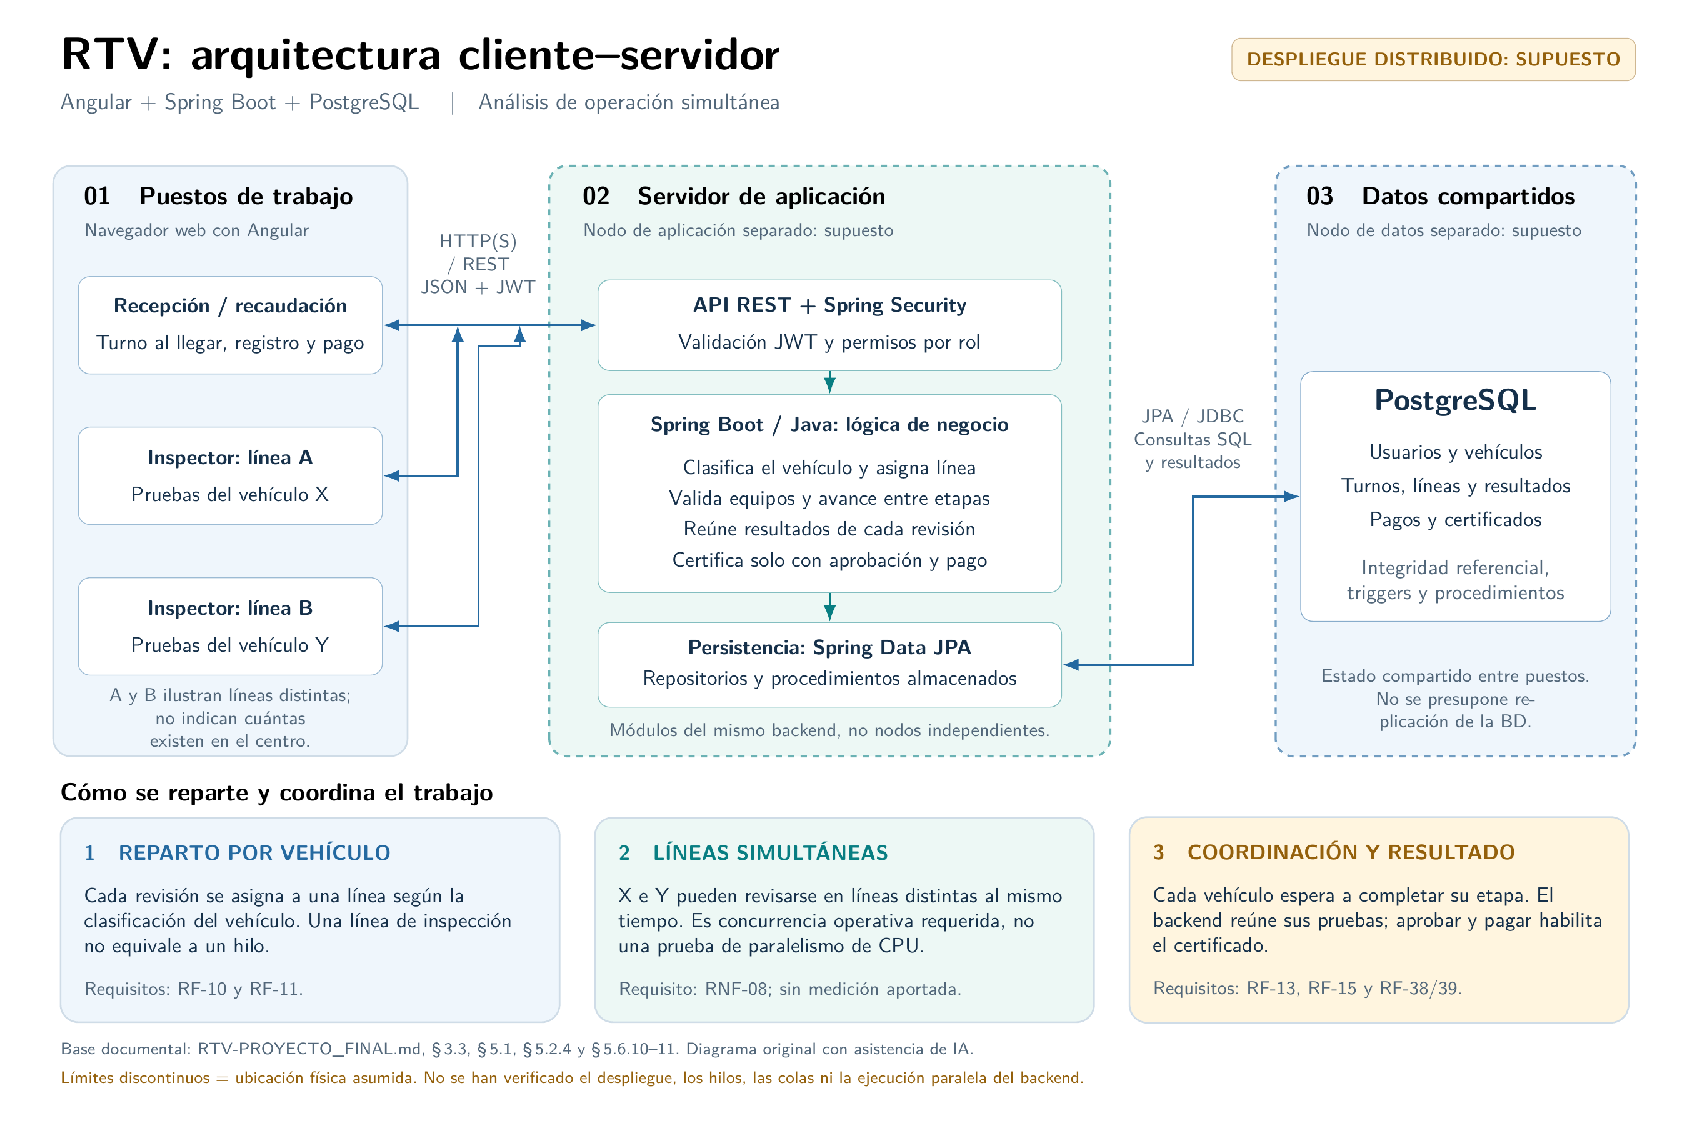
\includegraphics[width=\textwidth,height=4.35cm,keepaspectratio]{figuras/gs_arquitectura_resumen.pdf}
  \par\vspace{0.08cm}
  \raggedright
  {\small \textbf{Reparto:} por vehículo y línea. \quad
  \textbf{Reunión:} resultados de cada revisión.\par}
  \vspace{0.10cm}
  {\scriptsize Límites discontinuos: nodos físicos asumidos, no despliegue comprobado.\\
  Los módulos del backend no son microservicios. Un puesto no equivale a un hilo.\\
  Fuentes: documento RTV, \S\,3.3 y RF-10/11/15 \cite{gs_rtv};
  vocabulario REST: \cite{gs_spring_servlet}.}
\end{frame}

\begin{frame}{Dos revisiones concurrentes; cada una avanza en orden}
  \vspace{-0.10cm}
  \centering
  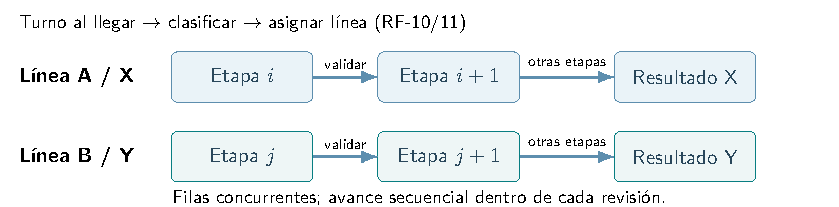
\includegraphics[width=\textwidth,height=3.2cm,keepaspectratio]{figuras/gs_recorrido.pdf}
  \par\vspace{0.05cm}
  \raggedright
  \begin{columns}[T,onlytextwidth]
    \begin{column}{0.49\textwidth}
      \begin{block}{Qué debe esperar}
        \small Etapa completa + equipo válido.\\
        Certificado: aprobado \textbf{y} pagado.
      \end{block}
    \end{column}
    \begin{column}{0.47\textwidth}
      \begin{block}{Qué no se ha demostrado}
        \small Hilos, aceleración o correo asíncrono.\\
        MVCC no sustituye las reglas del negocio.
      \end{block}
    \end{column}
  \end{columns}
  \vfill
  {\scriptsize Ejemplo ilustrativo: A/B y X/Y no son cifras de operación. Etapas genéricas, no tiempos reales.\\
  Fuentes: RNF-08, RF-13/24/25/38/39 \cite{gs_rtv}; MVCC \cite{gs_postgresql17}.}
\end{frame}

\begin{frame}{4. Transparencias durante el trabajo paralelo}
  En la práctica utilizamos \texttt{parallelize()} para distribuir cuatro vehiculos en dos y cuatro particiones.

  \begin{itemize}
    \item Transparencia ofrecida: Spark distribuye los datos y genera las tareas sin que tengamos que asignar manualmente cada vehiculo.
    \item Transparencia no completa: la distribucion y ejecucion interna no se muestran en la salida normal del programa. Para observarlas utilizamos Spark UI.
  \end{itemize}

  Comprobamos las particiones, los Jobs, los Stages y las Tasks desde la interfaz web.

  \par
\end{frame}

\begin{frame}{5. Comunicacion que coordina tareas}
  La practica se ejecuto en modo local mediante \texttt{local[*]}.

  \begin{itemize}
    \item Spark mostro un executor identificado como \texttt{driver}, con 12 cores disponibles.
    \item Al utilizar dos particiones observamos dos tareas completadas.
    \item Con cuatro particiones observamos cuatro tareas completadas.
    \item En el Event Timeline las tareas comenzaron aproximadamente al mismo tiempo.
  \end{itemize}

  La practica permitio observar la coordinacion de tareas en modo local, pero no comprobo la comunicacion entre nodos de un cluster ni un protocolo de mensajes.

  \par
\end{frame}

\begin{frame}{6. Espera y avance de tareas}
  Para recuperar los resultados utilizamos la accion \texttt{collect()}, que espera la ejecucion de las operaciones pendientes y devuelve los resultados al programa principal.

  \begin{itemize}
    \item Las tareas finalizaron correctamente: 2 de 2 y 4 de 4.
    \item El Event Timeline mostro intervalos de ejecucion superpuestos.
    \item No implementamos acciones asincronas ni barreras de sincronizacion.
  \end{itemize}

  Tambien medimos el tiempo de ejecucion. Con dos particiones obtuvimos un promedio de 1.8195 segundos y con cuatro particiones 3.4206 segundos.

  \par
\end{frame}

% HERRERA BARCO — sustituir marcadores antes de la entrega
\begin{frame}{7. Partición durante el trabajo paralelo}
  \begin{itemize}
    \item \textbf{Qué parte guarda el estado:} hay un componente que organiza el trabajo (reparte tareas y lleva el control de qué terminó y qué resultados intermedios hay) \cite{elhmadany2024,vandongen2021}.
    \item \textbf{Si algunos nodos quedan aislados:}
      \begin{itemize}
        \item lo que no se puede confirmar \textit{falla o se detiene};
        \item lo que depende de resultados pendientes \textit{se queda en espera};
        \item cuando es posible, \textit{se vuelve a intentar} en otros recursos \cite{vandongen2021,javed2023}.
      \end{itemize}
    \item \textbf{CAP (para esta parte):} se cuida que el avance sea correcto, aunque por un momento no pueda seguir avanzando \cite{vandongen2021,javed2023}.
  \end{itemize}
  {\footnotesize Se analiza este componente, no todo Spark ni otros servicios externos.}
\end{frame}

\begin{frame}{8. Estado y latencia sin partición}
  \begin{itemize}
    \item \textbf{Cómo se mantiene el orden:} el trabajo avanza por etapas y, antes de seguir, espera tener los resultados intermedios completos y correctos \cite{elhmadany2024,vandongen2021}.
    \item \textbf{Costo de coordinar:} repartir tareas, esperar y mover datos entre etapas toma tiempo, pero ayuda a que el resultado sea confiable \cite{mostafaei2022,elhmadany2024}.
    \item \textbf{PACELC (para esta parte):} sin partición, suele importar más que el resultado salga bien, aunque tarde un poco más \cite{vandongen2021,javed2023}.
    \item \textbf{Límite:} Spark tiene varias piezas; aquí se describe lo que se observa en la coordinación de la ejecución.
  \end{itemize}
\end{frame}

\begin{frame}{9. Comparación de sistemas de cómputo paralelo}
  \begin{table}
    \centering
    \scriptsize
    \begin{tabular}{@{}p{0.22\linewidth}p{0.35\linewidth}p{0.35\linewidth}@{}}
      \toprule
      \textbf{Punto} & \textbf{Apache Spark} & \textbf{Apache Flink} \\
      \midrule
      Cómo reparte el trabajo & Por tareas y etapas que se completan por partes \cite{elhmadany2024,vandongen2021}. & Como un flujo continuo de tareas conectadas \cite{javed2023}. \\
      Cómo se coordina & Espera a terminar etapas antes de pasar a las que dependen \cite{elhmadany2024}. & Controla el estado de forma continua y usa puntos de guardado \cite{javed2023}. \\
      Si algo falla & Vuelve a calcular partes perdidas \cite{vandongen2021,javed2023}. & Retoma usando el estado guardado \cite{javed2023}. \\
      A tener en cuenta & Coordinar y mover datos entre etapas puede tomar tiempo \cite{mostafaei2022,elhmadany2024}. & Manejar el estado puede ser más complejo según el caso \cite{javed2023}. \\
      \bottomrule
    \end{tabular}
  \end{table}
  \vspace{0.2em}
  {\footnotesize \textbf{Ejemplo RTV:} importa que cada etapa quede bien registrada antes del certificado (p.ej. RF-13, RF-24/25, RF-38/39, RNF-05). No se atribuye CAP/PACELC al RTV.}
\end{frame}

% LOMBEIDA ESCALERAS: Spark es el sistema analizado; RTV es el PFC.
\begin{frame}{10. Spark: recuperar trabajo paralelo}
  \vspace{0.28cm}
  {\large\bfseries Spark reintenta tareas y reconstruye datos perdidos.}\,\cite{sparkConfiguration,sparkRddGuide,sparkFetchFailed}\par
  \vspace{0.60cm}
  \begin{columns}[T,onlytextwidth]
    \begin{column}{0.31\textwidth}
      \begin{block}{Tarea fallida}
        Reintento limitado\,\cite{sparkConfiguration}
      \end{block}
    \end{column}
    \begin{column}{0.31\textwidth}
      \begin{block}{Partición RDD perdida}
        Recalcular por linaje\,\cite{sparkRddGuide}
      \end{block}
    \end{column}
    \begin{column}{0.31\textwidth}
      \begin{block}{Salida shuffle ausente}
        Regenerar datos previos\,\cite{sparkFetchFailed}
      \end{block}
    \end{column}
  \end{columns}
  \vspace{0.48cm}
  {\small\color{textoSuave}La recuperación depende del dato perdido y del tipo de fallo.\,\cite{sparkRddGuide,sparkFetchFailed}}
\end{frame}

\begin{frame}{11. Spark: un fallo real de recuperación}
  {\small\color{textoSuave}SPARK-46182 · registrado en 2023\,\cite{spark46182}}\par
  \vspace{0.55cm}
  \begin{columns}[T,onlytextwidth]
    \begin{column}{0.31\textwidth}
      \begin{block}{1. Tarea termina}
        Crea nuevos bloques shuffle.\,\cite{spark46182}
      \end{block}
    \end{column}
    \begin{column}{0.31\textwidth}
      \begin{block}{2. Executor sale}
        La migración aún no los detecta.\,\cite{spark46182}
      \end{block}
    \end{column}
    \begin{column}{0.31\textwidth}
      \begin{block}{3. Datos perdidos}
        Se recalcula la partición.\,\cite{spark46182}
      \end{block}
    \end{column}
  \end{columns}
  \vspace{0.55cm}
  {\small\bfseries Causa raíz:} carrera entre el fin de la tarea y el retiro del executor.\,\cite{spark46182}
\end{frame}

\begin{frame}{12. Lecciones para RTV y conclusiones}
  \vspace{0.28cm}
  {\small\color{textoSuave}Propuestas de mejora para el RTV; no se afirma que ya estén implementadas.}\par
  \vspace{0.55cm}
  \begin{columns}[T,onlytextwidth]
    \begin{column}{0.47\textwidth}
      \begin{block}{1. Conservar el avance}
        Confirmar cada resultado antes de continuar.\,\cite{postgresTransactions}
      \end{block}
    \end{column}
    \begin{column}{0.47\textwidth}
      \begin{block}{2. Cerrar sin perder datos}
        Verificar el estado completo antes de certificar.\,\cite{spark46182,postgresTransactions}
      \end{block}
    \end{column}
  \end{columns}
  \vspace{0.60cm}
  {\small\bfseries Idea final:} atender vehículos a la vez exige conservar íntegro el resultado de cada uno.\,\cite{spark46182,postgresTransactions}
\end{frame}


% Diapositiva de respaldo: no contar dentro de los 12 minutos.
\begin{frame}[allowframebreaks]{Referencias}\printbibliography[heading=none]\end{frame}
\end{document}
